%%%%%%%%%%%%%%%%%%%%%%%%%%%%%%%%%%%%%%%%%%%%%%%%%%%%%%%%%%%%%%%
% Welcome to the MAT320 Homework template on Overleaf -- just edit your
% LaTeX on the left, and we'll compile it for you on the right.
%%%%%%%%%%%%%%%%%%%%%%%%%%%%%%%%%%%%%%%%%%%%%%%%%%%%%%%%%%%%%%%
% --------------------------------------------------------------
% Based on a homework template by Dana Ernst.
% --------------------------------------------------------------
% This is all preamble stuff that you don't have to worry about.
% Head down to where it says "Start here"
% --------------------------------------------------------------

\documentclass[12pt]{article}

\usepackage{graphicx}
\graphicspath{{./images/}}
\usepackage[margin=1in]{geometry} 
\usepackage{amsmath,amsthm,amssymb}
% https://tex.stackexchange.com/questions/146306/how-to-make-horizontal-lists
\usepackage[inline]{enumitem} % allows using letters in enumerate list environment

% source: https://stackoverflow.com/questions/3175105/inserting-code-in-this-latex-document-with-indentation

\usepackage{listings}
\usepackage{color}

\definecolor{dkgreen}{rgb}{0,0.6,0}
\definecolor{gray}{rgb}{0.5,0.5,0.5}
\definecolor{mauve}{rgb}{0.58,0,0.82}

\lstset{frame=tb,
	language=C, % language for code listing
	aboveskip=3mm,
	belowskip=3mm,
	showstringspaces=false,
	columns=flexible,
	basicstyle={\small\ttfamily},
	numbers=none,
	numberstyle=\tiny\color{gray},
	keywordstyle=\color{blue},
	commentstyle=\color{dkgreen},
	stringstyle=\color{mauve},
	breaklines=true,
	breakatwhitespace=true,
	tabsize=4
}

\newcommand{\N}{\mathbb{N}}
\newcommand{\Z}{\mathbb{Z}}

\newenvironment{ex}[2][Exercise]{\begin{trivlist}
		\item[\hskip \labelsep {\bfseries #1}\hskip \labelsep {\bfseries #2.}]}{\end{trivlist}}

\newenvironment{sol}[1][Solution]{\begin{trivlist}
		\item[\hskip \labelsep {\bfseries #1:}]}{\end{trivlist}}


\begin{document}

% --------------------------------------------------------------
%                         Start here
% --------------------------------------------------------------

\noindent Sergio Garcia Tapia \hfill

\noindent{\small Digital Design and Computer Architecture: RISC-V} \hfill 

\noindent\today

\begin{ex}{2.1}
	Write a Boolean Equation in sum-of-products canonical form for each of the truth tables below: \
	\begin{center}
		\begin{enumerate*}[label=(\alph*)]
			\item \
			\begin{tabular}{cc|c}
				A & B & Y \\
				\hline
				0 & 0 & 1 \\
				0 & 1 & 0 \\
				1 & 0 & 1 \\
				1 & 1 & 1 \\
			\end{tabular}
			\item \
			
			\begin{tabular}{ccc|c}
				A & B & C & Y \\
				\hline
				0 & 0 & 0 & 1\\
				0 & 0 & 1 & 0\\
				0 & 1 & 0 & 0\\
				0 & 1 & 1 & 0\\
				1 & 0 & 0 & 0\\
				1 & 0 & 1 & 0\\
				1 & 1 & 0 & 0\\
				1 & 1 & 1 & 1\\
			\end{tabular}
			\item \begin{tabular}{ccc|c}
				A & B & C & Y \\
				\hline
				0 & 0 & 0 & 1\\
				0 & 0 & 1 & 0\\
				0 & 1 & 0 & 1\\
				0 & 1 & 1 & 0\\
				1 & 0 & 0 & 1\\
				1 & 0 & 1 & 1\\
				1 & 1 & 0 & 0\\
				1 & 1 & 1 & 1\\
			\end{tabular}
			\item \begin{tabular}{cccc|c}
				A & B & C & D & Y \\
				\hline
				0 & 0 & 0 & 0 & 1\\
				0 & 0 & 0 & 1 & 1\\
				0 & 0 & 1 & 0 & 1\\
				0 & 0 & 1 & 1 & 1\\
				0 & 1 & 0 & 0 & 0\\
				0 & 1 & 0 & 1 & 0\\
				0 & 1 & 1 & 0 & 0\\
				0 & 1 & 1 & 1 & 0\\
				1 & 0 & 0 & 0 & 1\\
				1 & 0 & 0 & 1 & 0\\
				1 & 0 & 1 & 0 & 1\\
				1 & 0 & 1 & 1 & 0\\
				1 & 1 & 0 & 0 & 0\\
				1 & 1 & 0 & 1 & 0\\
				1 & 1 & 1 & 0 & 1\\
				1 & 1 & 1 & 1 & 0\\
			\end{tabular}
			\item \
			
			\begin{tabular}{cccc|c}
				A & B & C & D & Y \\
				\hline
				0 & 0 & 0 & 0 & 1\\
				0 & 0 & 0 & 1 & 0\\
				0 & 0 & 1 & 0 & 0\\
				0 & 0 & 1 & 1 & 1\\
				0 & 1 & 0 & 0 & 0\\
				0 & 1 & 0 & 1 & 1\\
				0 & 1 & 1 & 0 & 1\\
				0 & 1 & 1 & 1 & 0\\
				1 & 0 & 0 & 0 & 0\\
				1 & 0 & 0 & 1 & 1\\
				1 & 0 & 1 & 0 & 1\\
				1 & 0 & 1 & 1 & 0\\
				1 & 1 & 0 & 0 & 1\\
				1 & 1 & 0 & 1 & 0\\
				1 & 1 & 1 & 0 & 0\\
				1 & 1 & 1 & 1 & 1\\
			\end{tabular}
		\end{enumerate*}
	\end{center}
\end{ex}

\begin{sol} \
	\begin{enumerate}[label=(\alph*)]
		\item $Y=\bar{A}\bar{B}+A\bar{B}+AB$
		\item $Y=\bar{A}\bar{B}\bar{C}+ABC$
		\item $Y=\bar{A}\bar{B}\bar{C}+\bar{A}B\bar{C}+A\bar{B}\bar{C}+A\bar{B}C+ABC$
		\item $Y=\bar{A}\bar{B}\bar{C}\bar{D}+\bar{A}\bar{B}\bar{C}D+\bar{A}\bar{B}C\bar{D}+\bar{A}\bar{B}CD+A\bar{B}\bar{C}\bar{D}+A\bar{B}C\bar{D}+ABCD\bar{D}$
		\item $\bar{A}\bar{B}\bar{C}\bar{D}+\bar{A}\bar{B}CD+\bar{A}B\bar{C}D+\bar{A}BC\bar{D}+A\bar{B}\bar{C}D+A\bar{B}C\bar{D}+AB\bar{C}\bar{D}+ABCD$
	\end{enumerate}
\end{sol}

\begin{ex}{2-3}
	Write a Boolean equation in product-of-sums canonical form for the truth tables in Exercise 2-1.
\end{ex}

\begin{sol} \
	\begin{enumerate}[label=(\alph*)]
		\item $Y=A+\bar{B}$
		\item $Y=(A+B+\bar{C})(A+\bar{B}+C)(A+\bar{B}+\bar{C})(\bar{A}+B+C)(\bar{A}+B+\bar{C})(\bar{A}+\bar{B}+C)$
		\item $Y=(A+B+\bar{C})(A+\bar{B}+\bar{C})(\bar{A}+\bar{B}+C)$
		\item $Y=(A+\bar{B}+C+D)(A+\bar{B}+C+\bar{D})(A+\bar{B}+\bar{C}+D)(A+\bar{B}+\bar{C}+\bar{D})(\bar{A}+B+C+\bar{D})(\bar{A}+B+\bar{C}+\bar{D})(\bar{A}+\bar{B}+C+D)(\bar{A}+\bar{B}+C+\bar{D})(\bar{A}+\bar{B}+\bar{C}+\bar{D})$
		\item $Y=(A+B+C+\bar{D})(A+B+\bar{C}+D)(A+\bar{B}+C+D)(A+\bar{B}+\bar{C}+\bar{D})(\bar{A}+B+C+D)(\bar{A}+B+\bar{C}+\bar{D})(\bar{A}+\bar{B}+C+\bar{D})(\bar{A}+\bar{B}+\bar{C}+D)$
	\end{enumerate}
\end{sol}

\begin{ex}{2-5}
	Minimize each of the Boolean equations from Exercise 2-1.
\end{ex}

\begin{sol}\
	
	\begin{enumerate}[label=(\alph*)]
		\item The K-map is shown in Figure~\ref{02-05a}. To minimize $Y=\bar{A}\bar{B}+A\bar{B}+AB$, we notice from the K-map that the minterm $A\bar{B}$ is shared, so we use the idempotency to duplicate it and use it in simplification:
		\[
		Y=\bar{A}\bar{B}+A\bar{B}+AB=(\bar{A}\bar{B}+A\bar{B})+(A\bar{B}+AB)=\bar{B}+A
		\]
		\begin{figure}
			\centering
			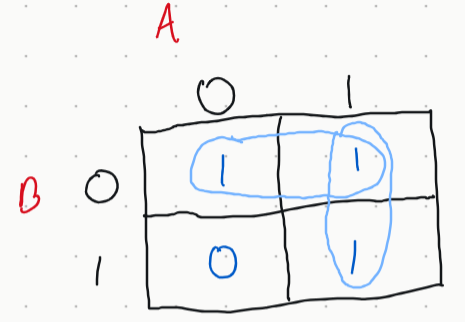
\includegraphics[width=0.4\textwidth]{02-05a-k-map}
			\caption{Exercise 2.5 (a): K-Map for Truth Table in Exercise 2-1 (a)}
			\label{02-05a}
		\end{figure}
		\item The K-map is shown in Figure ~\ref{02-05b}. It shows that the implicants in $Y=\bar{A}\bar{B}\bar{C}+ABC$ are prime implicants and hence, the equation cannot be reduced further.
		\begin{figure}
			\centering
			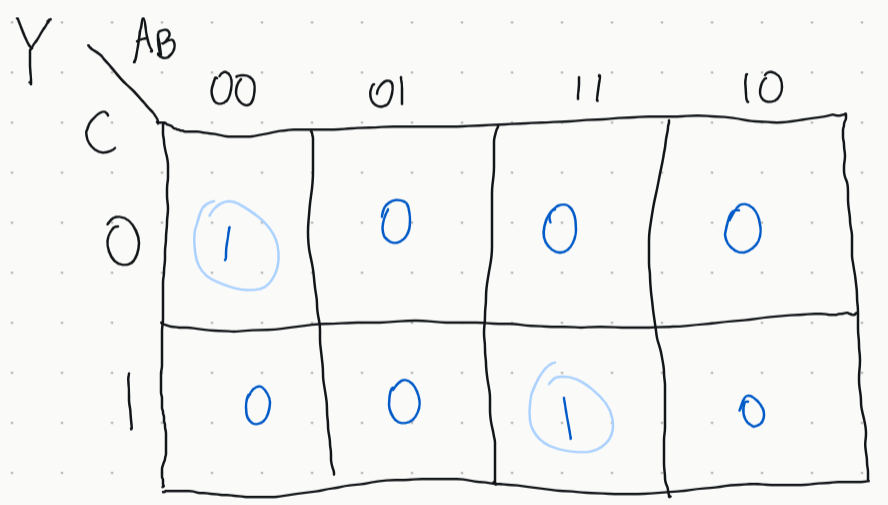
\includegraphics[width=0.4\textwidth]{02-05b-k-map}
			\caption{Exercise 2.5 (b): K-Map for Truth Table in Exercise 2-1 (b)}
			\label{02-05b}
		\end{figure}
		\item The K-map is shown in Figure~\ref{02-05c}. It reveals that
		$Y=\bar{A}\bar{B}\bar{C}+\bar{A}B\bar{C}+A\bar{B}\bar{C}+A\bar{B}C+ABC$ can be reduced:
		\begin{align}
			Y&=\bar{A}\bar{B}\bar{C}+\bar{A}B\bar{C}+A\bar{B}\bar{C}+A\bar{B}C+ABC\nonumber\\
			&=(\bar{A}\bar{B}\bar{C}+\bar{A}B\bar{C})+(A\bar{B}\bar{C}+A\bar{B}C)+(A\bar{B}C+ABC)\nonumber\\
			&=\bar{A}\bar{C}+A\bar{B}+AC\nonumber
		\end{align}
		\begin{figure}
			\centering
			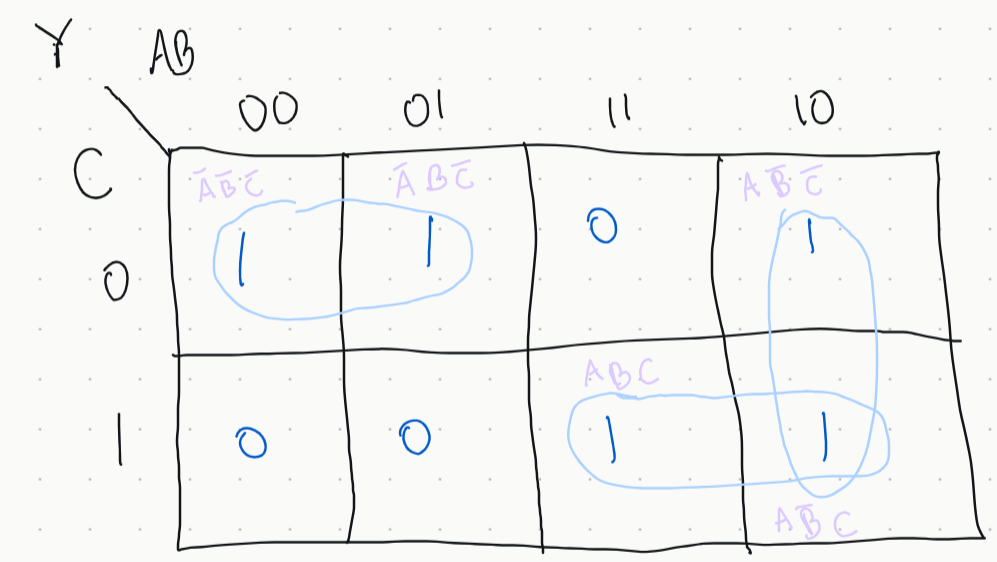
\includegraphics[width=0.4\textwidth]{02-05c-k-map}
			\caption{Exercise 2.5 (c): K-Map for Truth Table in Exercise 2-1 (c)}
			\label{02-05c}
		\end{figure}
		\item The K-map is shown in Figure~\ref{02-05d}. It reveals how to reduce the equation $Y=\bar{A}\bar{B}\bar{C}\bar{D}+\bar{A}\bar{B}\bar{C}D+\bar{A}\bar{B}C\bar{D}+\bar{A}\bar{B}CD+A\bar{B}\bar{C}\bar{D}+A\bar{B}C\bar{D}+ABCD\bar{D}$. First we work with the implicants belonging to the rectangle of size 4 in the first column:
		\begin{align}
			(
			(\bar{A}\bar{B}\bar{C}\bar{D}+\bar{A}\bar{B}\bar{C}D)
			+(\bar{A}\bar{B}CD+\bar{A}\bar{B}C\bar{D})
			)
			=(\bar{A}\bar{B}\bar{C})+(\bar{A}\bar{B}C)
			=(\bar{A}\bar{B})\nonumber
		\end{align}
		Then we work with the other 4-by-4 rectangle that wraps around:
		\begin{align}
			(\bar{A}\bar{B}\bar{C}\bar{D}+A\bar{B}\bar{C}\bar{D})
			+(\bar{A}\bar{B}C\bar{D}+A\bar{B}C\bar{D})
			=\bar{B}\bar{C}\bar{D}+\bar{B}C\bar{D}
			=\bar{B}\bar{D}\nonumber
		\end{align}
		Finally, we work with the 2-by-2 square that shares a minterm
		$A\bar{B}C\bar{D}$:
		\[
		ABC\bar{D}+A\bar{B}C\bar{D}=AC\bar{D}
		\]
		Altogether, the minimized equation is $Y=AC\bar{D}+\bar{A}\bar{B}+\bar{B}\bar{D}$.
		\begin{figure}
			\centering
			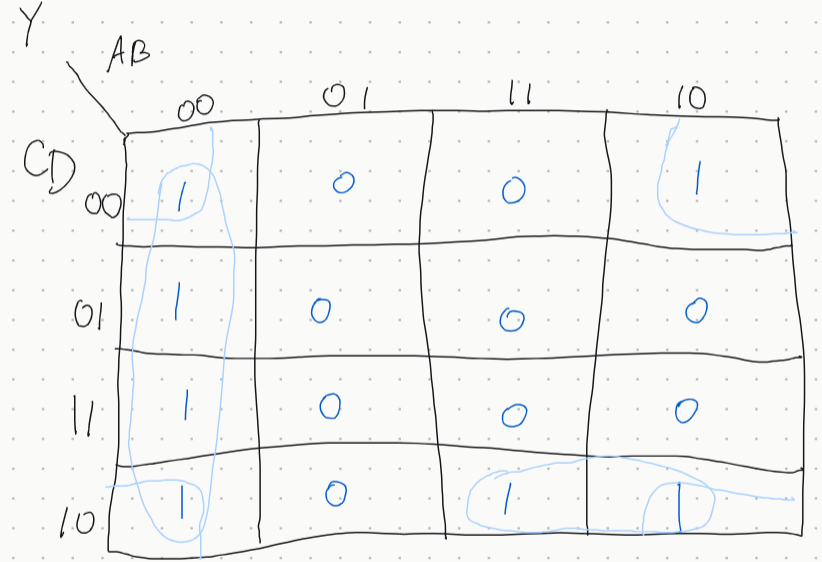
\includegraphics[width=0.4\textwidth]{02-05d-k-map}
			\caption{Exercise 2.5 (d): K-Map for Truth Table in Exercise 2-1 (d)}
			\label{02-05d}
		\end{figure}
		\item The K-Map is shown in Figure~\ref{02-05e}. It reveals that it is not possible to reduce sum, so $Y=\bar{A}\bar{B}\bar{C}\bar{D}+\bar{A}\bar{B}CD+\bar{A}B\bar{C}D+\bar{A}BC\bar{D}+A\bar{B}\bar{C}D+A\bar{B}C\bar{D}+AB\bar{C}\bar{D}+ABCD$.
		\begin{figure}
			\centering
			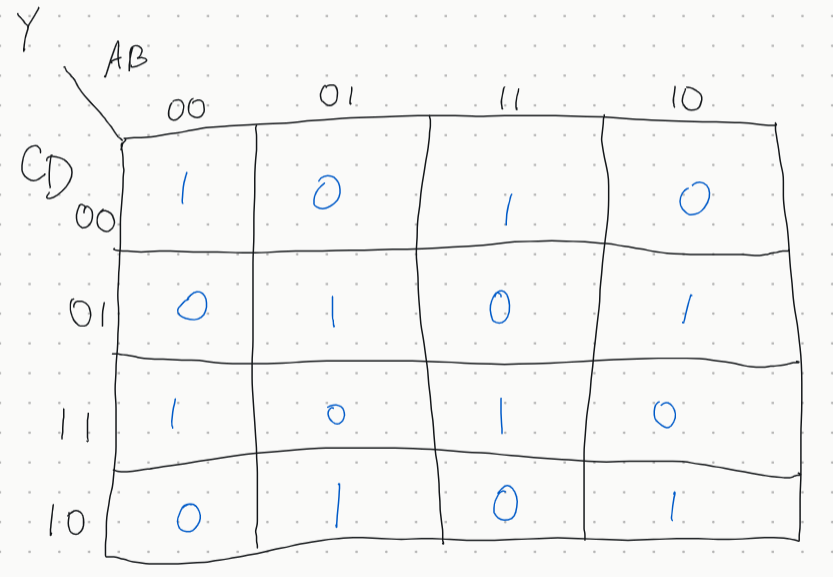
\includegraphics[width=0.4\textwidth]{02-05e-k-map}
			\caption{Exercise 2.5 (e): K-Map for Truth Table in Exercise 2-1 (e)}
			\label{02-05e}
		\end{figure}
	\end{enumerate}
\end{sol}

\begin{ex}{2.7}
	Sketch a reasonably simple combinational circuit implementing each of the functions from Exercise 2.5. \emph{Reasonably simple} means that you are not wasteful of gates, but you don't waste vast amounts of time checking every possible combination of the circuit either.
\end{ex}

\begin{sol}
	\begin{enumerate}[label=(\alph*)]
		\item See Figure~\ref{02-07a}.
		\begin{figure}
			\centering
			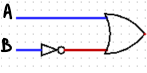
\includegraphics[width=0.4\textwidth]{02-07a-circuit}
			\caption{Exercise 2.7 (a): Circuit implementing boolean equation in Exercise 2.5(a)}
			\label{02-07a}
		\end{figure}
		\item See Figure~\ref{02-07b}. See Figure~\ref{02-07b-alt} for an alternative.
		\begin{figure}
			\centering
			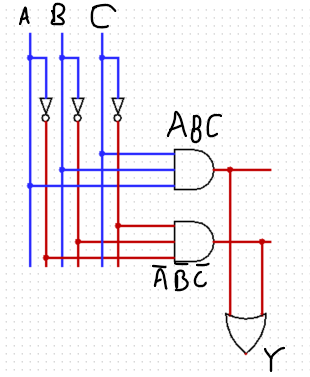
\includegraphics[width=0.4\textwidth]{02-07b-circuit}
			\caption{Exercise 2.7 (b): Circuit implementing boolean equation in Exercise 2.5(b)}
			\label{02-07b}
		\end{figure}
		\begin{figure}
			\centering
			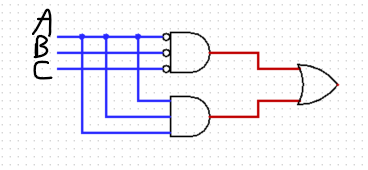
\includegraphics[width=0.4\textwidth]{02-07b-circuit-alternate}
			\caption{Exercise 2.7 (b) - Alternnative: Circuit implementing boolean equation in Exercise 2.5(b)}
			\label{02-07b-alt}
		\end{figure}
		\item Note that $\bar{A}\bar{C}+AC$ corresponds to the following 2-input truth table, which shows it is equivalent to a NOT gate followed by an XOR gate, which is a XNOR gate.
		\begin{center}
			\begin{tabular}{cc|c}
				A & C & Y \\
				\hline
				0 & 0 & 1 \\
				0 & 1 & 0 \\
				1 & 0 & 0 \\
				1 & 1 & 1 \\
			\end{tabular}
		\end{center}
		With that in mind, the circuit is given in Figure~\ref{02-07c}
		\begin{figure}
			\centering
			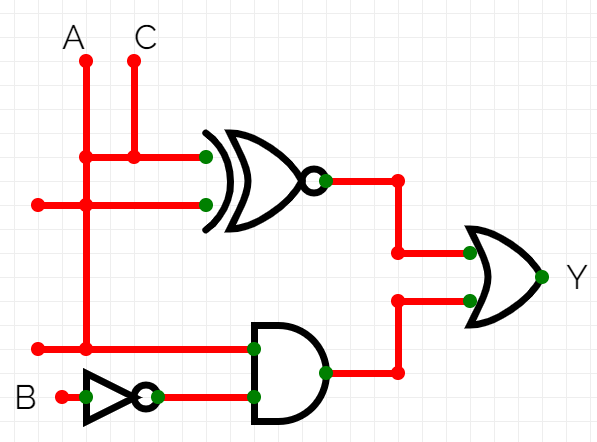
\includegraphics[width=0.4\textwidth]{02-07c-circuit}
			\caption{Exercise 2.7 (c): Circuit implementing boolean equation in Exercise 2.5 (c)}
			\label{02-07c}
		\end{figure}
		\item See Figure~\ref{02-07d}
			\begin{figure}
			\centering
			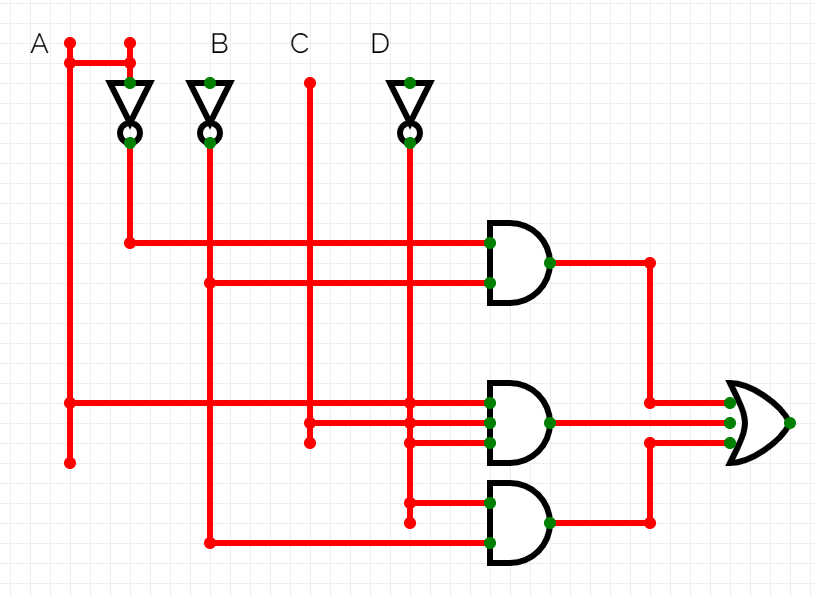
\includegraphics[width=0.4\textwidth]{02-07d-circuit}
			\caption{Exercise 2.7 (d): Circuit implementing boolean equation in Exercise 2.5 (d)}
			\label{02-07d}
		\end{figure}
		\item From the truth corresponding to Exercise 2.5 (e), and hence Exercise 2.1 (e), the output is 1 when there is an even number of 1s, or when we have all 0s. This is the opposite of an XOR gate, which is 1 when an odd number of inputs are 1. Hence, this is the negation of a 4-input NOR gate. According to section 2.5.1 in the book, we can build a XOR gate from using
		cascading XOR gates. Therefore, we can use two XOR gates and one XNOR gate. See Figure~\ref{02-07e}
		
		\begin{figure}
			\centering
			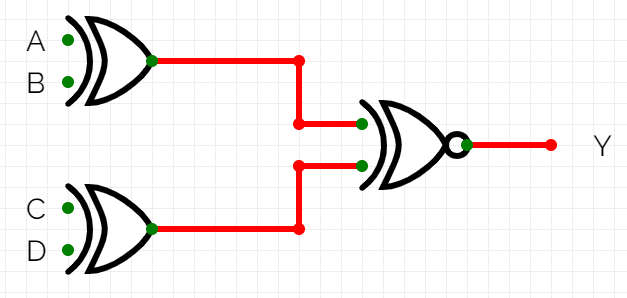
\includegraphics[width=0.4\textwidth]{02-07e-circuit}
			\caption{Exercise 2.7 (e): Circuit implementing boolean equation in Exercise 2.5 (e)}
			\label{02-07e}
		\end{figure}
	\end{enumerate}
\end{sol}

\begin{ex}{2.9}
	Repeat Exercise 2.7 using only NOT gates, and AND, and OR gates.
	\begin{enumerate}[label=(\alph*)]
		\item Same as Exercise 2.5 (a), which is in Figure~\ref{02-05a}.
		\item Same as version 1 of Exercise 2.5(b), which is in Figure~\ref{02-07b}.
		\item See Figure~\ref{02-09c}.
		\begin{figure}
			\centering
			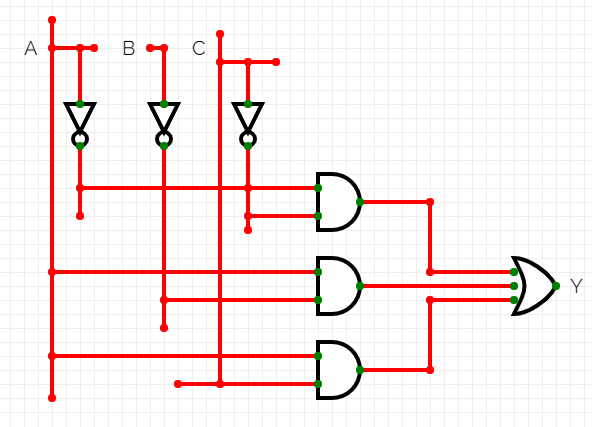
\includegraphics[width=0.4\textwidth]{02-09c-circuit}
			\caption{Exercise 2.9 (c): Circuit implementing boolean equation in Exercise 2.5 (c) using only AND, OR, NOT}
			\label{02-09c}
		\end{figure}
		\item We can write the equation as
		$Y=\bar{D}(AC+\bar{B})+\bar{A}\bar{B}$. See Figure~\ref{02-09d}.
		\begin{figure}
			\centering
			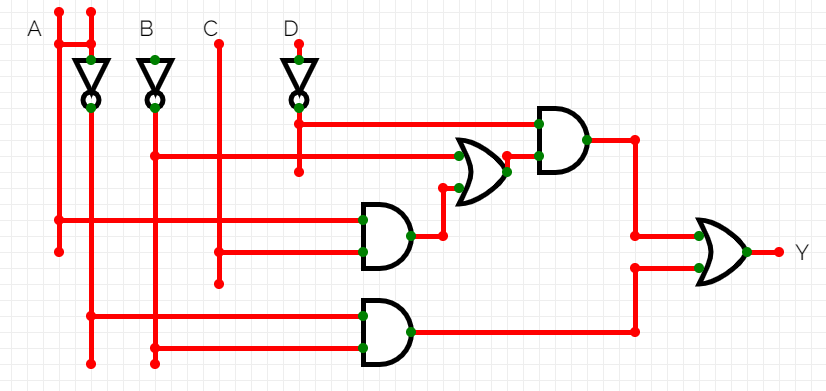
\includegraphics[width=0.4\textwidth]{02-09d-circuit}
			\caption{Exercise 2.9 (d): Circuit implementing boolean equation in Exercise 2.5 (d) using only AND, OR, NOT}
			\label{02-09d}
		\end{figure}
		\item We can use the distributive property to re-write the equation as:
		\begin{align}
			Y&=\bar{A}\bar{B}\bar{C}\bar{D}+\bar{A}\bar{B}CD+\bar{A}B\bar{C}D+\bar{A}BC\bar{D}+A\bar{B}\bar{C}D+A\bar{B}C\bar{D}+AB\bar{C}\bar{D}+ABCD
			\nonumber\\
			&=(\bar{A}\bar{B})(\bar{C}\bar{D}+CD)
			+(\bar{A}B)(\bar{C}D+C\bar{D})
			+(A\bar{B})(\bar{C}D+C\bar{D})
			+(AB)(\bar{C}\bar{D}+CD)\nonumber\\
			&=(\bar{A}\bar{B}+AB)(\bar{C}\bar{D}+CD)+
			(\bar{A}B+A\bar{B})(\bar{C}D+C\bar{D})\nonumber
		\end{align}
		Alternatively, note that:
		\begin{align*}
			\overline{(\bar{A}\bar{B}+AB)}&=
			(A+B)(\bar{A}+\bar{B})\qquad\text{(De Morgan's Theorem)}\\
			&=A\bar{A}+A\bar{B}+B\bar;{A}+B\bar{B}\\
			&=A\bar{B}+\bar{A}B
		\end{align*}
		Using this, we could further simplify our equation. Letting $G=\bar{A}\bar{B}+AB$ and
		$H=\bar{C}\bar{D}+CD$, we can write $Y$ as:
		\[
		Y=HG+\bar{H}\bar{G}
		\]
		See Figure~\ref{02-09e}.
		\begin{figure}
			\centering
			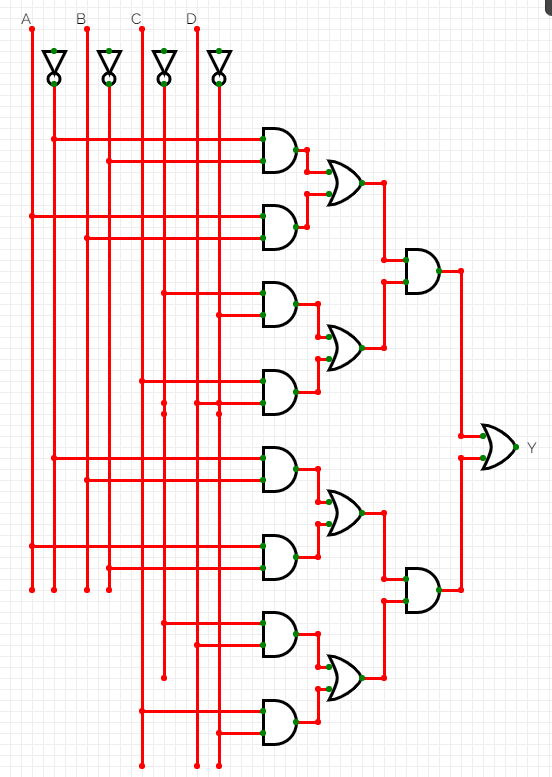
\includegraphics[width=0.4\textwidth]{02-09e-circuit}
			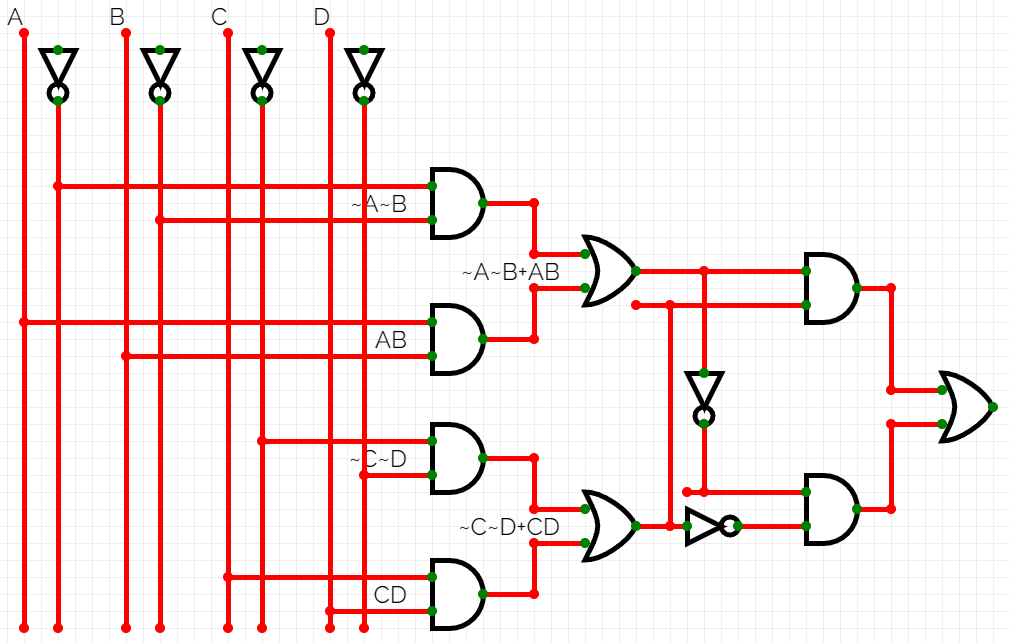
\includegraphics[width=0.4\textwidth]{02-09e-circuit-alternate}
			\caption{Exercise 2.9 (e): Two Circuits implementing boolean equation in Exercise 2.5 (e) using only AND, OR, NOT}
			\label{02-09e}
		\end{figure}
	\end{enumerate}
\end{ex}

\begin{ex}{2.11}
	Repeat Exercise 2.7 using only NOT and NAND and NOR gates.
\end{ex}

\begin{sol}
	\begin{enumerate}[label=(\alph*)]
		\item The equation $Y=\bar{B}+A$ is equivalent to $Y=\bar{B\bar{A}}$. This implies the circuit in
		Figure~\ref{02-11a}.
		\begin{figure}
			\centering
			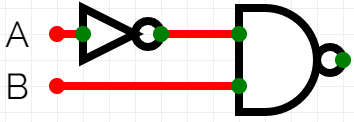
\includegraphics[width=0.3\textwidth]{02-11a-circuit}
			\caption{Exercise 2.11 (a): Circuit implementing boolean equation in $Y=\bar{B}+A$ with only NAND and NOT}
			\label{02-11a}
		\end{figure}
		\item We can brute force it by replacing AND gates with NAND and NOT, and OR gates with NOR and NOT. Then we simplify and get Figure~\ref{02-11b}
		\begin{figure}
			\centering
			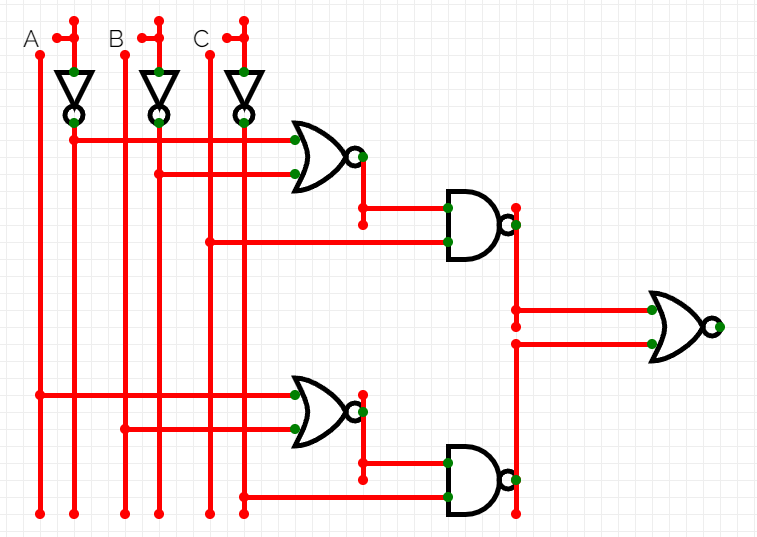
\includegraphics[width=0.3\textwidth]{02-11b-circuit}
			\caption{Exercise 2.11 (b): Circuit implementing $Y=\bar{A}\bar{B}\bar{C}+ABC$ using only NOT, NAND, and NOR gates.}
			\label{02-11b}
		\end{figure}
		\item The equation is $Y=\bar{A}\bar{C}+A\bar{B}+AC$.
		\begin{figure}
			\centering
			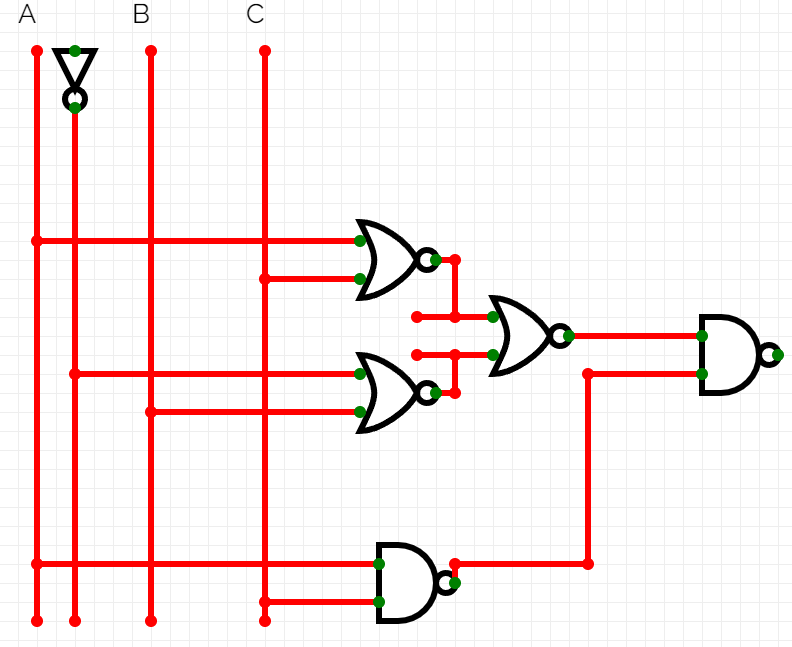
\includegraphics[width=0.3\textwidth]{02-11c-circuit}
			\caption{Exercise 2.11 (c): Circuit implementing $Y=\bar{A}\bar{C}+A\bar{B}+AC$. using only NOT, NAND, and NOR gates.}
			\label{02-11c}
		\end{figure}
		\item The equation is 	$Y=\bar{D}(AC+\bar{B})+\bar{A}\bar{B}$.
		\begin{figure}
			\centering
			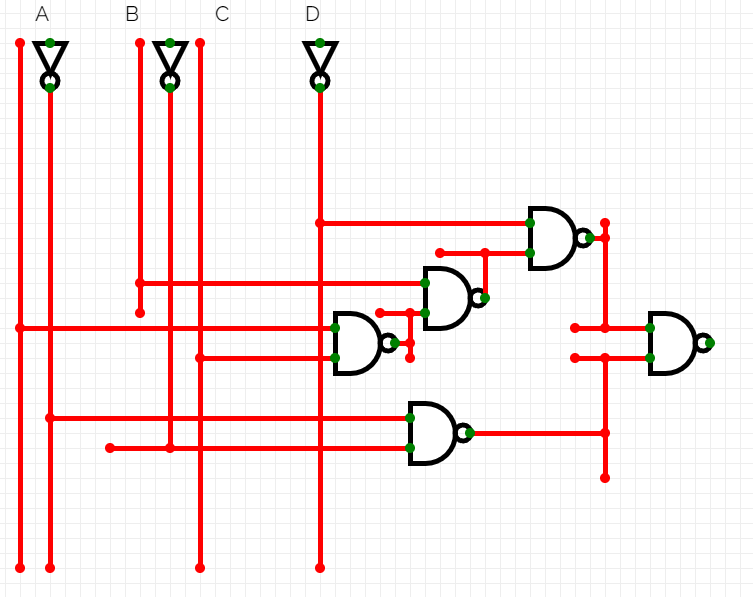
\includegraphics[width=0.3\textwidth]{02-11d-circuit}
			\caption{Exercise 2.11 (d): Circuit implementing $Y=\bar{A}\bar{C}+A\bar{B}+AC$. using only NOT, NAND, and NOR gates.}
			\label{02-11d}
		\end{figure}
		\item See Figure~\ref{02-11e}
		\begin{figure}
			\centering
			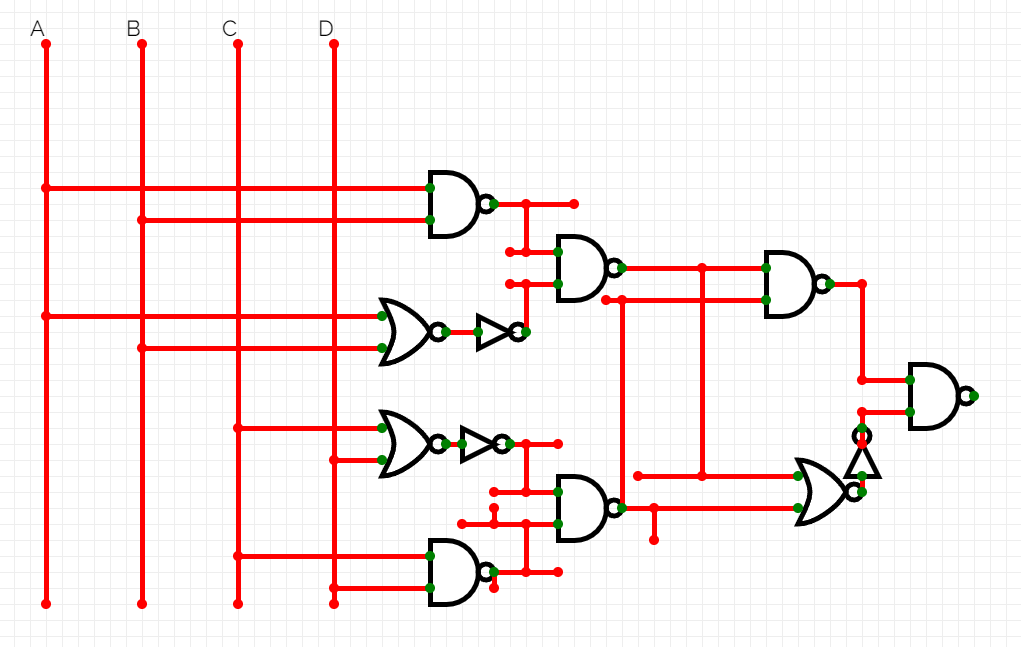
\includegraphics[width=0.3\textwidth]{02-11e-circuit}
			\caption{Exercise 2.11 (e): Circuit implementing $Y=\bar{A}\bar{C}+A\bar{B}+AC$. using only NOT, NAND, and NOR gates.}
			\label{02-11e}
		\end{figure}
	\end{enumerate}
\end{sol}

\begin{ex}{2.19}
	Give an example of a truth table requiring between 3 billion and 5 billion rows that can be constructed using fewer than 40 (but at least 1) two-input gates.
\end{ex}

\begin{sol}
	Consider the 32-input AND boolean function:
	\[
	Y=\prod_{n=1}^{32}A_n
	\]
	There are $2^{32}$ outputs (around 4.3 billion).
	It can be constructed with 31 two-input AND gates.
\end{sol}

\begin{ex}{2.21}
	Alyssa P. Hacker says that any Boolean function can be written in minimal sum-of-product form as the sum of all of the prime implicants of the function.
	Ben Bitdiddle says there are some funnctions whose minimal equation
	does not involve all of the prime implicants. Explain why Alyssa is right or
	proved a counterexample demonstrating Ben's point.
\end{ex}

\begin{sol}
	Alyssa is not correct. Consider Figure~\ref{2-21-kmaps}, representing
	a K-Map for a boolean equation that is reduced in two ways:
	\begin{align*}
		Y&=A\bar{B}\bar{C}D+\bar{A}B\bar{C}D+AB\bar{C}D+\bar{A}BCD+\bar{A}BC\bar{D}\\
		Y&=\bar{A}BC\bar{D}+\bar{A}B\bar{C}D+\bar{A}BCD+AB\bar{C}D+A\bar{B}\bar{C}D
	\end{align*}
	We can now reduce them to (respectively):
	\begin{align*}
		Y&=A\bar{B}\bar{C}D+B\bar{C}D+\bar{A}BC\\
		Y&=\bar{A}BC\bar{D}+\bar{A}BD+A\bar{C}D
	\end{align*}
	Note that both of this equations are minimal, and both contain distinct prime implicants.
	\begin{figure}
		\centering
		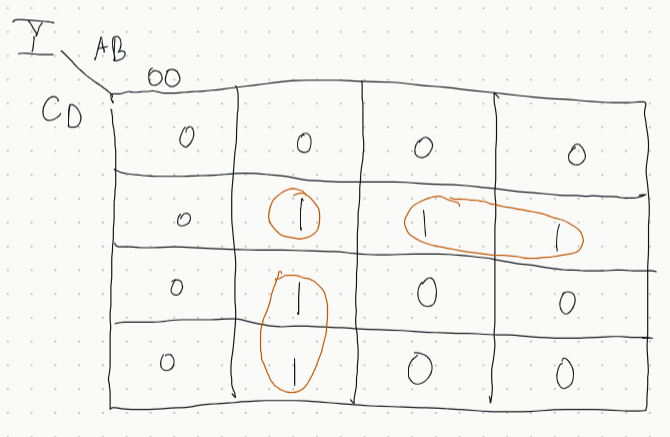
\includegraphics[width=0.4\textwidth]{02-21-kmap-min1}
		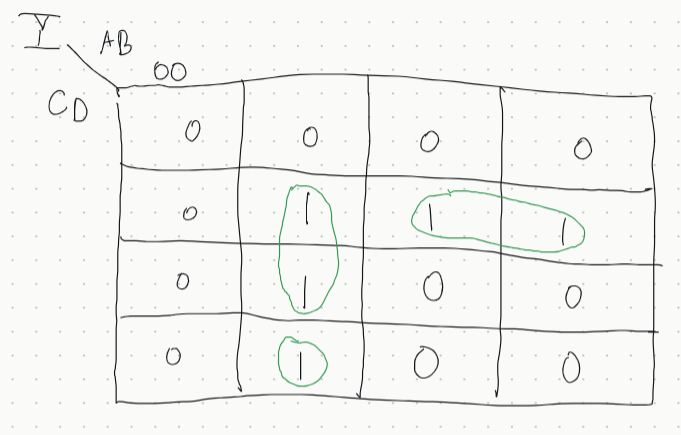
\includegraphics[width=0.4\textwidth]{02-21-kmap-min2}
		\caption{2-21: K-Map for two equivalent, minimal boolean equations}
		\label{2-21-kmaps}
	\end{figure}
\end{sol}

\begin{ex}{2.22}
	Prove the following theorems are true using perfect induction.
	You need not prove their duals.
	\begin{enumerate}[label=(\alph*)]
		\item The idempotency theorem (T3)
		\item The distributivity theorem (T8)
		\item The combining theorem (T10)
	\end{enumerate}
\end{ex}

\begin{sol}
	\begin{enumerate}[label=(\alph*)]
		\item Idempotency says that $B\cdot B=B$. If $B=0$, then equation says $0\cdot 0=0$, which is a true equation. If $B=1$, then it says $1\cdot 1 =1$, which is also a true equation.
		\item Distributivity says $(B\cdot C)+(B\cdot D)=B\cdot (C+D)$.
		Consider the truth tables:
		\begin{center}
			\begin{tabular}{ccc|c|c}
				$B$ & $C$ & $D$ & $(B\cdot C)+(B\cdot D)$ & $B\cdot (C+D)$\\
				\hline
				0 & 0 & 0 & 0 & 0\\
				0 & 0 & 1 & 0 & 0\\
				0 & 1 & 0 & 0 & 0\\
				0 & 1 & 1 & 0 & 0\\
				1 & 0 & 0 & 0 & 0\\
				1 & 0 & 1 & 1 & 1\\
				1 & 1 & 0 & 1 & 1\\
				1 & 1 & 1 & 1 & 1\\
			\end{tabular}
		\end{center}
		\item Combining theorem says: $(B\cdot C)+(B\cdot \bar{C})=B$.
		The truth table is as follows:
		\begin{center}
			\begin{tabular}{cc|c}
				$C$ & $B$ & $(B\cdot C)+(B\cdot \bar{C})$\\
				\hline
				0 & 0 & 0\\
				0 & 1 & 1\\
				1 & 0 & 0\\
				1 & 1 & 1\\
			\end{tabular}
		\end{center}
	\end{enumerate}
\end{sol}

\begin{ex}{2.23}
	Prove De Morgan's Theorem for three variables, A, B, and C, using perfect induction.
\end{ex}

\begin{sol}
	De Morgan's says that
	\[
	\overline{\prod B_n}=\sum \bar{B_n}
	\]
	There are two cases:
	\begin{enumerate}
		\item 	Suppose that a term $B_k$ is 0. Then the left-hand product
		is 0, and the inverse operation makes the result 1. On the right-hand
		side, since $B_k=0$, it follows that $\bar{B_k}=1$, and since
		the right-hand side consists of OR operations only, the entire result
		becomes 1. Hence, both sides are 1.
		\item Suppose that no term is 0. That is, every $Bn$ is 1. The
		product is 1, and the inverse is 0, meaning the left-hand side is 0.
		For the right-hand side, since every $B_n$, it follows that every
		$\bar{B_n}$ is 0, and the OR of them all is still 0. Hence, both sides
		are 0.
	\end{enumerate}

\end{sol}

\begin{ex}{2.24}
	Write Boolean equations for the circuit in Figure 2.82 (in the book, page 98).
	You need not minimize the equations.
\end{ex}

\begin{sol}
	The equations are:
	\begin{align*}
		Y&=\bar{A}D+A\bar{C}D+A\bar{B}C+ABCD\\
		Z&=BD+A\bar{C}D
	\end{align*}
\end{sol}

\begin{ex}{2.25}
	Minimize the Boolean Equations from Exercise 2.24 and sketch an improved
	circuit with the same function.
\end{ex}

\begin{sol}
	The following is the boolean table for this function:
	\begin{center}
		\begin{tabular}{cccc|c}
			$A$ & $B$ & $C$ & $D$ & $Y$\\
			\hline
			0 & 0 & 0 & 0 & 0\\
			0 & 0 & 0 & 1 & 1\\
			0 & 0 & 1 & 0 & 0\\
			0 & 0 & 1 & 1 & 1\\
			0 & 1 & 0 & 0 & 0\\
			0 & 1 & 0 & 1 & 1\\
			0 & 1 & 1 & 0 & 0\\
			0 & 1 & 1 & 1 & 1\\
			1 & 0 & 0 & 0 & 0\\
			1 & 0 & 0 & 1 & 1\\
			1 & 0 & 1 & 0 & 1\\
			1 & 0 & 1 & 1 & 1\\
			1 & 1 & 0 & 0 & 0\\
			1 & 1 & 0 & 1 & 1\\
			1 & 1 & 1 & 0 & 0\\
			1 & 1 & 1 & 1 & 1\\
		\end{tabular}
	\end{center}
	The corresponding K-Map is in Figure~\ref{02-25-kmap}.
	\begin{figure}
		\centering
		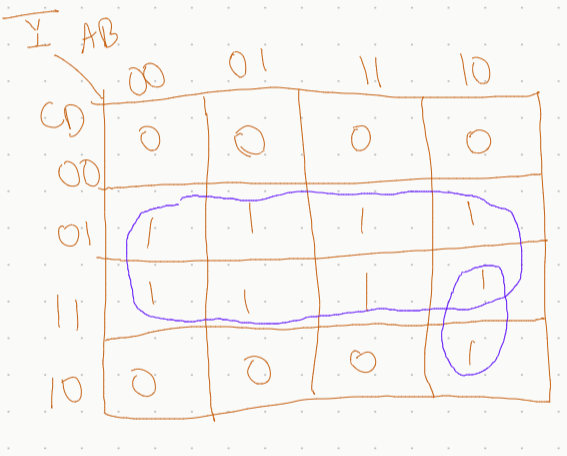
\includegraphics[width=0.5\textwidth]{02-25-kmap}
		\caption{Exercise 2-25: Boolean table for boolean function on
			Exercise 2-23}
		\label{02-25-kmap}
	\end{figure}
	We have a prime implicant consisting of 8 minterms, and a
	prime implicant with one minterm:
	\begin{align*}
		Y&=\bar{A}\bar{B}\bar{C}D+\bar{A}\bar{B}CD
		+\bar{A}B\bar{C}D+\bar{A}BCD+AB\bar{C}D+ABCD
		+A\bar{B}\bar{C}D+A\bar{B}CD
		+A\bar{B}C\bar{D}\\
		Y&=\bar{A}\bar{B}D+\bar{A}BD+ABD+A\bar{B}D+A\bar{B}C\bar{D}\\
		Y&=\bar{A}D+AD+A\bar{B}C\bar{D}\\
		Y&=D+A\bar{B}C\bar{D}
	\end{align*}
	The improved circuit can be seen on Figure~\ref{02-25-circuit}.
	\begin{figure}
		\centering
		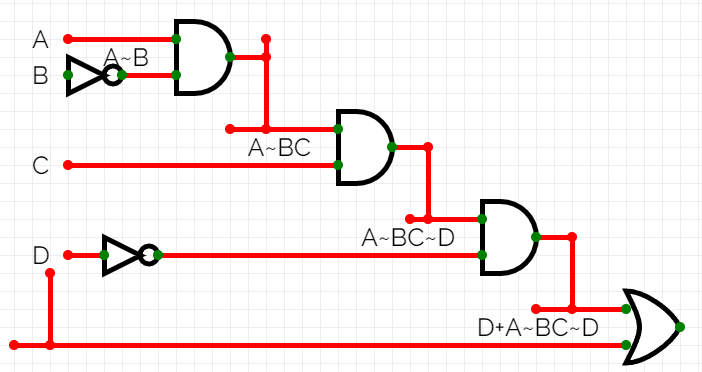
\includegraphics[width=0.4\textwidth]{02-25-improved-circuit}
		\caption{Exercise 2-25: Improved version of the circuit in Exercise 2.24.}
		\label{02-25-circuit}
	\end{figure}
\end{sol}

\begin{ex}{2.26}
	Using De Morgan equivalent gates and bubble pushing methods, redraw
	the circuit in Figure~\ref{02-26-circuit-original} so that you can
	find the Boolean equation by inspection. Write the Boolean equation.
	\begin{figure}
		\centering
		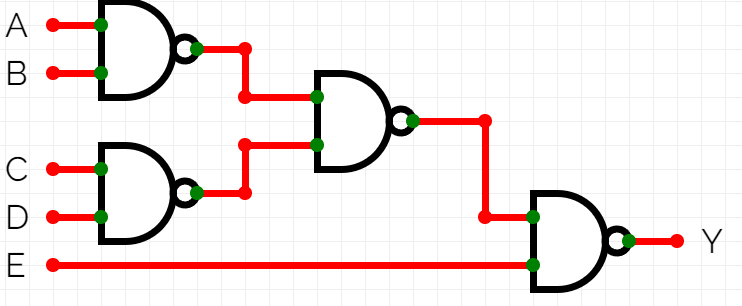
\includegraphics[width=0.4\textwidth]{02-26-circuit-original}
		\caption{Exercise 2-26: Original circuit to reduce}
		\label{02-26-circuit-original}
	\end{figure}
\end{ex}

\begin{sol}
	The re-written circuit is in Figure~\ref{02-26-circuit-demorgan-equivalent}.
	The boolean equation can be written as:
	\[
	Y=\bar{A}\bar{B}\bar{C}\bar{D}+\bar{E}
	\]
	\begin{figure}
		\centering
		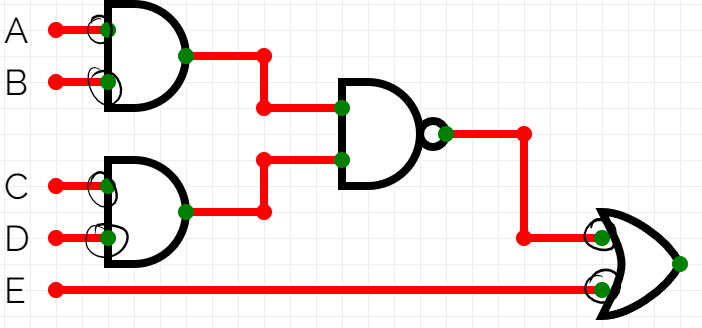
\includegraphics[width=0.4\textwidth]{02-26-circuit-demorgan-equivalent}
		\caption{Exercise 2-26: Re-written circuit}
		\label{02-26-circuit-demorgan-equivalent}
	\end{figure}
\end{sol}

\begin{ex}{2.27}
	Repeat Exercise 2.26 for the circuit in Figure~\ref{02-27-circuit-original}.
	\begin{figure}
		\centering
		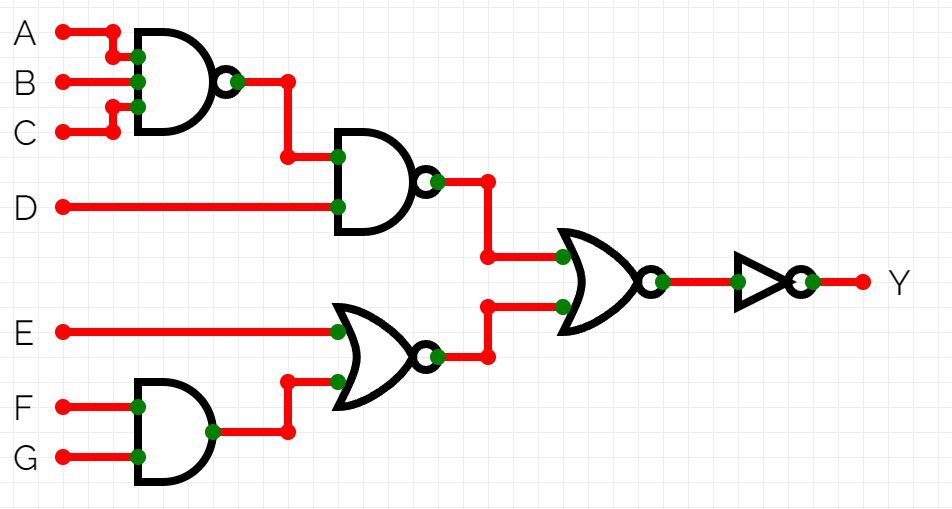
\includegraphics[width=0.4\textwidth]{02-27-circuit-original}
		\caption{Exercise 2-27: Circuit to rewrite}
		\label{02-27-circuit-original}
	\end{figure}
\end{ex}

\begin{sol}
	The rewritten circuit is in Figure~\ref{02-27-circuit-rewritten}.
	\[
	Y=(ABC+\bar{D})+(\bar{E}(\bar{F}+\bar{G}))
	\]
	\begin{figure}
		\centering
		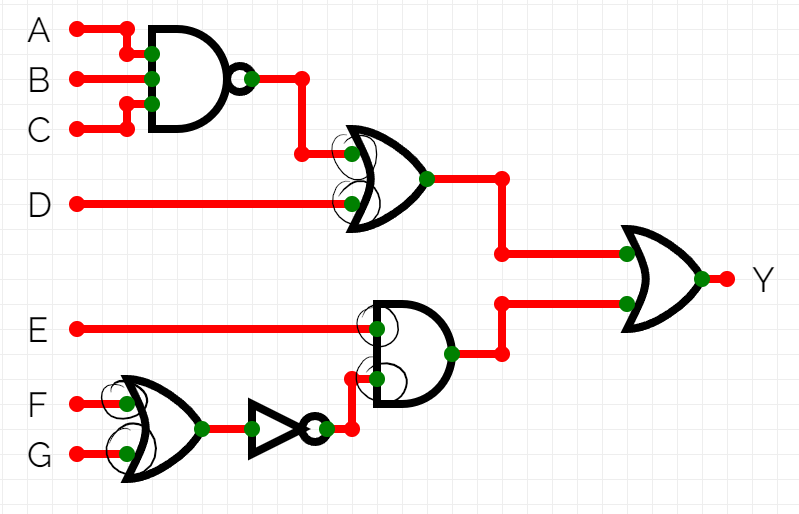
\includegraphics[width=0.4\textwidth]{02-27-circuit-rewritten}
		\caption{Exercise 2-27: Rewritten version}
		\label{02-27-circuit-rewritten}
	\end{figure}
\end{sol}

\begin{ex}{2.28}
	Find a minimal Boolean equation for the function in the table below.
	Remember to take advantage of the  don't care entries.
	\begin{center}
		\begin{tabular}{cccc|c}
			$A$ & $B$ & $C$ & $D$ & $Y$\\
			\hline
			0 & 0 & 0 & 0 & X\\
			0 & 0 & 0 & 1 & X\\
			0 & 0 & 1 & 0 & X\\
			0 & 0 & 1 & 1 & 0\\
			0 & 1 & 0 & 0 & 0\\
			0 & 1 & 0 & 1 & X\\
			0 & 1 & 1 & 0 & 0\\
			0 & 1 & 1 & 1 & X\\
			1 & 0 & 0 & 0 & 1\\
			1 & 0 & 0 & 1 & 0\\
			1 & 0 & 1 & 0 & X\\
			1 & 0 & 1 & 1 & 1\\
			1 & 1 & 0 & 0 & 1\\
			1 & 1 & 0 & 1 & 1\\
			1 & 1 & 1 & 0 & X\\
			1 & 1 & 1 & 1 & 1\\
		\end{tabular}
	\end{center}
\end{ex}

\begin{sol}
	The corresponding K-Map is given in Figure~\ref{02-29-kmap-with-dont-cares}.
	\begin{figure}
		\centering
		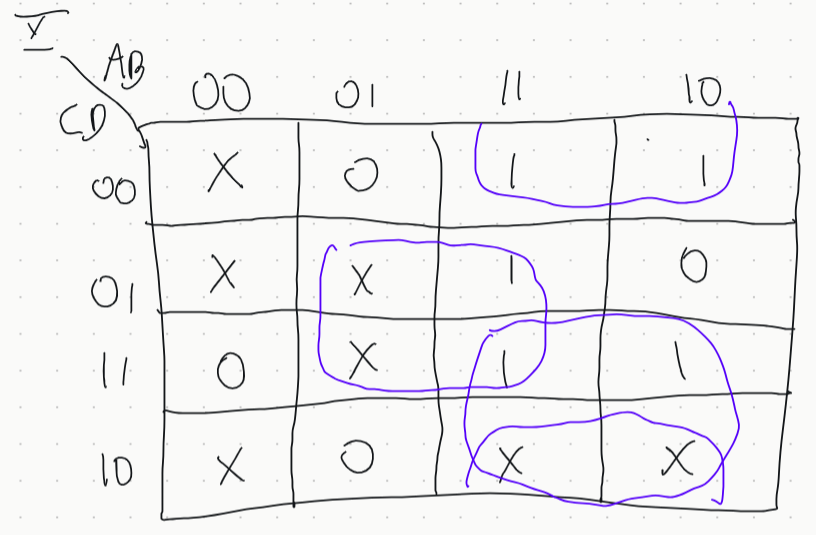
\includegraphics[width=0.4\textwidth]{02-29-kmap-with-dont-cares}
		\caption{Exercise 2-28: K-Map for truth table with don't cares}
		\label{02-29-kmap-with-dont-cares}
	\end{figure}
	The corresponding equation is:
	\begin{align*}
		Y&=\bar{A}B\bar{C}D+\bar{A}BCD+AB\bar{C}D+ABCD\\
		&+ABCD+A\bar{B}CD+ABC\bar{D}+A\bar{B}C\bar{D}\\
		&+AB\bar{C}\bar{D}+A\bar{B}\bar{C}\bar{D}+ABC\bar{D}+A\bar{B}C\bar{D}\\
		&=\bar{A}BD+ABD
		+ACD+AC\bar{D}
		+A\bar{C}\bar{D}+AC\bar{D}\\
		&=BD+AC+A\bar{D}
	\end{align*}
\end{sol}

\begin{ex}{2.29}
	Sketch a circuit for the function from Exercise 2.28.
\end{ex}

\begin{sol}
	See Figure~\ref{02-29circuit}
	\begin{figure}
		\centering
		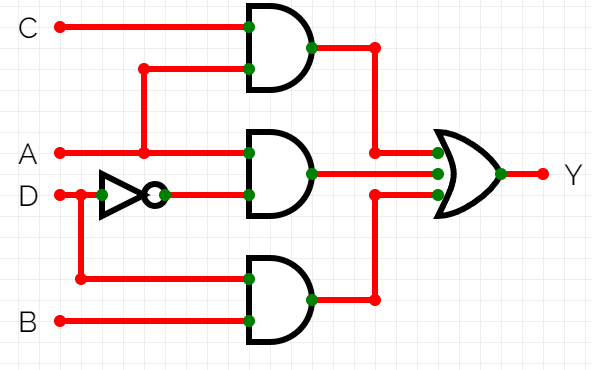
\includegraphics[width=0.4\textwidth]{02-29-circuit}
		\caption{Exercise 02-29: Circuit from Boolean function on Exercise 02-28}
		\label{02-29circuit}
	\end{figure}
\end{sol}

\begin{ex}{2.30}
	Does your circuit from Exercise 2.29 have any potential glitches when one of the inputs changes?
	If not, explain why not. If so, show how to
	modify the circuit to eliminate the glitches.
\end{ex}

\begin{sol}
	Yes, there is a glitch. Note in Figure~\ref{02-29-kmap-with-dont-cares}
	that there $AB\bar{C}\bar{D}$ and $AB\bar{C}D$ belong to different
	prime implicants, but if $D$ changes from 0 to 1, or from 1 to 0, the
	boundary between the implicants is crossed. In particular, consider
	the state of the system when $ABCD=1101$ (corresponding to the prime implicant $AB\bar{C}D$ just mentioned). See Figure~\ref{02-30glitched}.
	
	\begin{figure}
		\centering
		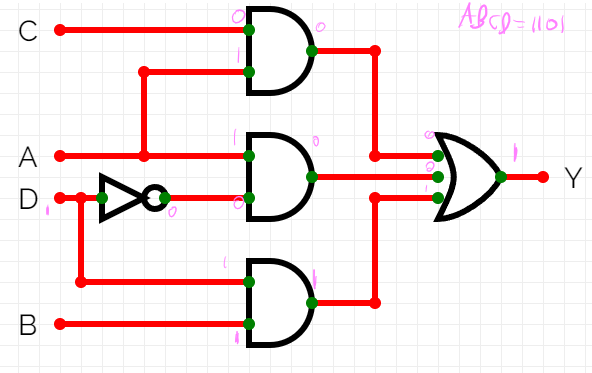
\includegraphics[width=0.4\textwidth]{02-30-preglitch-circuit}
		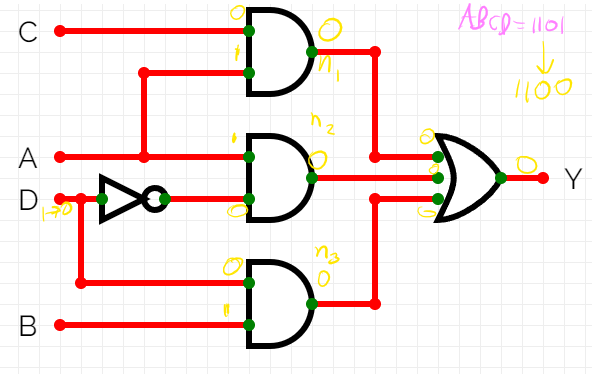
\includegraphics[width=0.4\textwidth]{02-30-transient-circuit}
		\caption{Exercise 02-30: Glitch across prime implicant boundary from ABCD=1101 to ABCD=1100.}
		\label{02-30glitched}
	\end{figure}
	
	In particular, node $n_3$ falls from 1 to 0 before $n_2$ rises from 0 to 1, 
	and thus there is a short time during which $Y$ has a value of $0$
	and not 1. To fix the issue, we add a circle to cover the prime implicant
	boundary. In doing so, we stretch it to cover all 4 squares on
	the third column. This makes the center square superflous so we remove it, and the updated K-Map is shown on Figure~\ref{02-30-updated-kmap}
	
	\begin{figure}
		\centering
		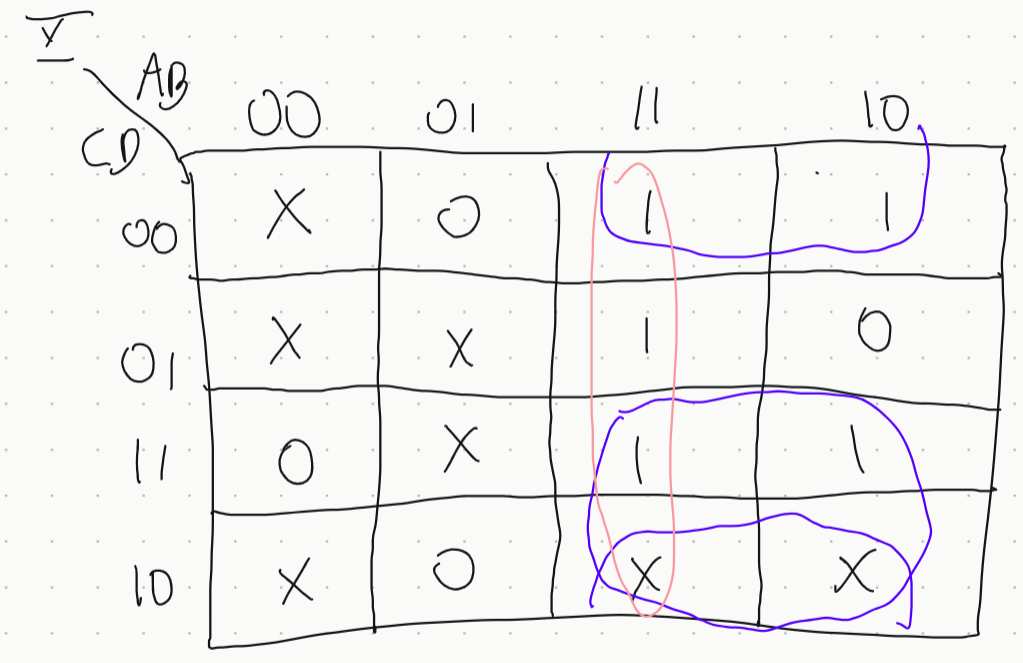
\includegraphics[width=0.4\textwidth]{02-30-updated-kmap}
		\caption{Exercise 02-30: Updated K-Map with no term crossing
		a prime implicant boundary.}
		\label{02-30-updated-kmap}
	\end{figure}
	Now we can simplify this updated K-Map:
	\begin{align*}
		Y&=AB\bar{C}\bar{D}+AB\bar{C}D+ABCD+ABC\bar{D}\\
		&+ABCD+A\bar{B}CD+ABC\bar{D}+A\bar{B}C\bar{D}\\
		&+ABC\bar{D}+A\bar{B}C\bar{D}+AB\bar{C}\bar{D}+A\bar{B}\bar{C}\bar{D}\\
		&=AB\bar{C}+ABC
		+ACD+AC\bar{D}
		+AC\bar{D}+A\bar{C}\bar{D}\\
		&=AB+AC+A\bar{D}\\
		&=A(B+C+\bar{D})
	\end{align*}
	The updated, glitch-less circuit is in Figure~\ref{02-30-updated-circuit-no-glitch}.
	\begin{figure}
		\centering
		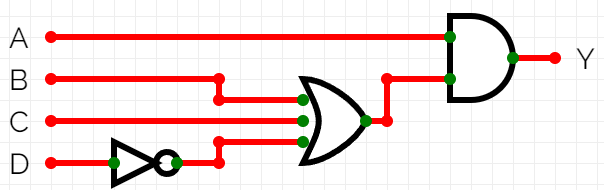
\includegraphics[width=0.4\textwidth]{02-30-updated-circuit-no-glitch}
		\caption{Exercise 02-30: Updated circuit without glitch}
		\label{02-30-updated-circuit-no-glitch}
	\end{figure}
\end{sol}

\begin{ex}{2.31}
	Find a minimal Boolean equation for the function
	in the Boolean table below.
	
		\begin{center}
		\begin{tabular}{cccc|c}
			$A$ & $B$ & $C$ & $D$ & $Y$\\
			\hline
			0 & 0 & 0 & 0 & 0\\
			0 & 0 & 0 & 1 & 1\\
			0 & 0 & 1 & 0 & X\\
			0 & 0 & 1 & 1 & X\\
			0 & 1 & 0 & 0 & 0\\
			0 & 1 & 0 & 1 & X\\
			0 & 1 & 1 & 0 & X\\
			0 & 1 & 1 & 1 & X\\
			1 & 0 & 0 & 0 & 1\\
			1 & 0 & 0 & 1 & 0\\
			1 & 0 & 1 & 0 & 0\\
			1 & 0 & 1 & 1 & 1\\
			1 & 1 & 0 & 0 & 0\\
			1 & 1 & 0 & 1 & 1\\
			1 & 1 & 1 & 0 & X\\
			1 & 1 & 1 & 1 & 1\\
		\end{tabular}
	\end{center}
	Remember to take advantage of the don't care entries.
\end{ex}

\begin{sol}
	\begin{align*}
		Y&=A\bar{B}\bar{C}\bar{D}\\
		&+\bar{A}\bar{B}\bar{C}D+\bar{A}B\bar{C}D+\bar{A}\bar{B}CD+\bar{A}BCD\\
		&+\bar{A}B\bar{C}D+\bar{A}BCD+AB\bar{C}D+ABCD\\
		&+\bar{A}\bar{B}CD+\bar{A}BCD+ABCD+A\bar{B}CD\\
		&=A\bar{B}\bar{C}\bar{D}
		+\bar{A}\bar{C}D+\bar{A}CD
		+\bar{A}BD+ABD
		+\bar{A}CD+ACD\\
		&=A\bar{B}\bar{C}\bar{D}
		+\bar{A}D+BD+CD
	\end{align*}
\end{sol}

\begin{ex}{2.32}
	Sketch a circuit for the function from Exercise 2.31
\end{ex}
 
\begin{sol}
	We can simplify the function further to 
	\[
	Y=A\bar{B}\bar{C}\bar{D}
	+D(\bar{A}+B+C)=\bar{D}A\bar{B}\bar{C}+D\overline{A\bar{B}\bar{C}}
	\]
	The corresponding circuit is on Figure~\ref{02-32-circuit}.
	\begin{figure}
		\centering
		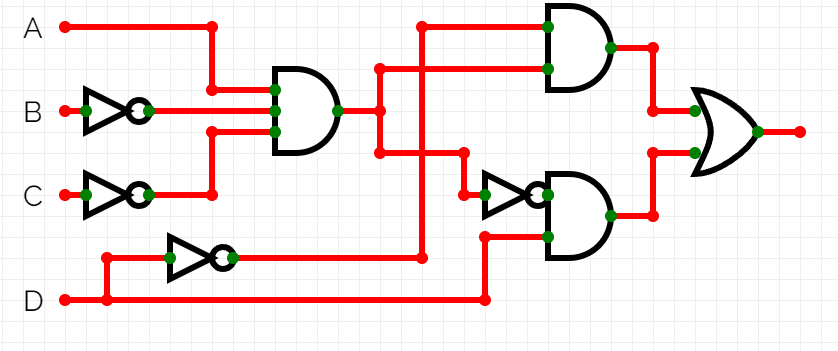
\includegraphics[width=0.4\textwidth]{02-32-circuit}
		\caption{Exercise 02-32: Circuit based on boolean table in
		Exercise 2-31.}
		\label{02-32-circuit}
	\end{figure}
\end{sol}

\begin{ex}{2.33}
	Ben Bitdiddle will enjoy his picnic on sunny days that have no ants.
	He will also enjoy his picnic any day he sees a hummingbird, as well as
	on days where there are ants and lady bugs. Write a Booelan equation
	for his enjoyment ($E$) in terms of sun ($S$), ants $(A)$,
	hummingbirds $(H)$, and ladybugs $(L)$.
\end{ex}

\begin{sol}
	\[
	E=S\bar{A}+H+AL
	\]
\end{sol}
\end{document}